\documentclass[12pt]{article}

\usepackage{scrextend}
\usepackage{sbc-template}
\usepackage{mathtools}
\usepackage{subfigure}
\usepackage{wrapfig}
\usepackage{graphicx,url}
\usepackage{booktabs}
\usepackage[brazil]{babel}   
\usepackage[utf8]{inputenc}
\usepackage{hhline}
\usepackage{enumitem, array}
\usepackage{boldline}
\usepackage{hyperref}
\usepackage{url}
\usepackage{relsize}
\usepackage{setspace}
\usepackage[T1]{fontenc} % hifenizar as palavras

\newcommand{\mn}[1]{\textcolor{red}{\bf [Michele]: #1}}

% algoritmo - pacote 9/out/2017
\usepackage[portuguese,ruled,noline,linesnumbered]{algorithm2e}

\let\oldnl\nl% Store \nl in \oldnl
\newcommand{\nonl}{\renewcommand{\nl}{\let\nl\oldnl}}% Remove line number for one line

%% Useful packages
\usepackage{mathtools}
\usepackage{graphicx}
\setlength{\marginparwidth}{2cm}
\usepackage[colorinlistoftodos]{todonotes}
\usepackage{multirow}
\usepackage{bigstrut}

\definecolor{ao(english)}{rgb}{0.0, 0.5, 0.0}

\renewcommand\thesubfigure{(\alph{subfigure})}

\newcommand{\notered}[1]{\textcolor{red}{{#1}}}
\newcommand{\noteblue}[1]{\textcolor{blue}{{\bf #1}}}
\newcommand{\as}[1]{\textcolor{blue}{{\bf #1}}}
\newcommand{\al}[1]{\textcolor{brown}{{\bf #1}}}
\newcommand{\noteMat}[1]{\textcolor{cyan}{{\bf #1}}}
\newcommand{\noteGreen}[1]{\textcolor{green}{{\bf #1}}}
\newcommand{\sep}{\hspace{8 mm}}
\newcommand{\pl}[1]{{\color{red}{[#1]}}}
\newcommand{\mnr}[1]{{\color{blue}{[Necessário corrigir/revisar:  #1]}}}
\newcommand{\co}[1]{{\color{magenta}{[Comentário:  #1]}}}
\newcommand{\mnc}[1]{{\color{brown}{[Comentário:  #1]}}}
\newcommand{\mic}[1]{\textcolor{magenta}{{\bf #1}}}

\newcommand{\agn}[1]{\textcolor{ao(english)}{{#1}}}
%\newcommand{\agn}[1]{\textcolor{black}{{#1}}}

\newcommand{\rev}[1]{\textcolor{black}{{#1}}}
%\newcommand{\rev}[1]{\textcolor{red}{{#1}}}

\usepackage{indentfirst}
\usepackage{verbatim}
\usepackage{amsmath}
\sloppy

\usepackage{array}
\usepackage{threeparttable}
\usepackage{listings}

\title{Disseminação Segura de Dados Pessoais Vitais Para Apoio às Tomadas de Decisão em Situações Emergenciais}


%NR2 – Programa de Pós-Graduação em Informática - UFPR
%NR2 – Programa de Pós-Graduação em Informática - UFPR –- Brasil
%NR2 – Programa de Pós-Graduação em Informática - UFPR –- Brasil
%NR2 – PPPGInf - Departamento de Informática – Universidade Federal do Paraná 
%NR2 – PPGInf - Depto. de Informática - Universidade Federal do Paraná -- UFPR 
%PPGInf - Núcleo de Redes Sem-Fio e Redes Avançadas (NR2) -- UFPR 
\author{Agnaldo de Souza Batista\inst{1}\thanks{{Dissertação de mestrado disponível em https://www.acervodigital.ufpr.br/handle/1884/62473}}\,\,, Aldri Santos\inst{1} (Orientador)} 
\address{Núcleo de Redes Sem-Fio e Redes Avançadas (NR2) -- PPGInf -- UFPR 
%-- Curitiba -- PR -- Brasil 
%\\
%\\ Universidade Federal do Paraná (UFPR)
%\\
%Caixa Postal 19.081 -- 81.531-980 
%-- Curitiba -- PR -- Brasil
\email{\{asbatista,aldri\}@inf.ufpr.br}
}


% adicionado por Aldri para fazer marcação d'agua de no. de versão do documento
\usepackage{xcolor}
\usepackage{xwatermark} 
\usepackage[export]{adjustbox}
%\newwatermark*[allpages,angle=60,scale=2,color=red!30,xpos=-10pt,ypos=10pt]{Rascunho}
%\newwatermark[allpages,scale=8,angle=60,xpos=-1.5cm,ypos=1cm]{\LaTeX}
%\newwatermark[allpages,scale=2,angle=60,xpos=-1.5cm,ypos=1cm]{Draft SBRC 2019}

% adicionado por Aldri para inclusão de comentários de pontos a ser melhorados ao longo do documento
%\newcommand{\notered}[1]{\textcolor{red}{[{\bf #1}]}}
%\newcommand{\noteblue}[1]{\textcolor{blue}{{\bf #1}}}
% adicionado por aldri
%\usepackage[inline]{trackchanges}
%\addeditor{FM}
%\addeditor{AS}
%\addeditor{JS}
%%\note[FM]{}

\usepackage{float}

\begin{document} 
\pagestyle{myheadings} % numerar páginas
\maketitle

\begin{abstract}
Urban wireless networks established dynamically have become possible the 
quick dissemination of a number of 
data, making them a promising means to support services that require a prompt response. Network health services (\textit{e-health}) that manage critical health events external to hospital environments and demand dissemination of sensitive personal data can benefit from interactions in these networks, collaborating in anticipating specific actions to be taken by trained people close to the events until the attendance by the competent health agencies. This dissertation presents STEALTH, a system that employs social trust~and communities of interest to control the dissemination of people's sensitive data in emergencies in dynamic environments. An evaluation of STEALTH under a realistic environment has shown its effectiveness in anticipating the identification of people close to assist in critical health events and the reliability for the dissemination of sensitive data of people in an emergency.

%The Urban networks dynamically established have made it possible to disseminate data quickly, making it a promising means of supporting services that require a prompt response. Network health services (\ textit {e-health}) that manage critical health events external to hospital environments and demand the dissemination of sensitive personal data can benefit from interactions in these networks, collaborating in anticipation of specific actions by trained people close to the events until the attendance by the competent health agencies. This dissertation presents STEALTH, a system that employs social trust and communities of interest in controlling the dissemination of people's sensitive data in emergencies in dynamic environments. An evaluation of STEALTH in a realistic environment showed its effectiveness in anticipating the identification of people close to assist in critical health events and its reliability in the controlled dissemination of sensitive data of people in an emergency.


\end{abstract}


\begin{resumo} 

As redes urbanas estabelecidas dinamicamente têm possibilitado a disseminação de dados de maneira rápida, tornando-se um meio promissor ao suporte de serviços que exigem pronta resposta. Os serviços de saúde em redes (\textit{e-health}) que gerenciam eventos críticos de saúde externos aos ambientes hospitalares e demandam a disseminação de dados pessoais sensíveis podem se beneficiar das interações nessas redes, colaborando na antecipação de certas ações por pessoas capacitadas próximas aos eventos até o atendimento pelos órgãos de saúde competentes. Esta dissertação apresenta o STEALTH, um sistema que emprega confiança social e comunidades de interesse no controle da disseminação dos dados sensíveis das pessoas em situações emergenciais em ambientes dinâmicos. Uma avaliação do STEALTH num ambiente realístico mostrou a sua eficácia ao antecipar a identificação de pessoas próximas para auxiliar em eventos críticos de saúde, e a sua confiabilidade na disseminação controlada dos dados sensíveis das pessoas em situação emergencial.

\begin{comment}

Resumo 4

Prover dados em ambientes sem infraestruturas de redes é um desafio. Nessas condições, redes estabelecidas dinamicamente muitas vezes viabilizam a disseminação dos dados, suportando serviços que exigem rápida resposta, como os serviços de saúde em redes (\textit{e-health}). Durante um evento crítico, quando uma pessoa sente-se mal, por exemplo, suas condições de saúde estão disponíveis até o seu atendimento pelos órgãos competentes. A eficácia desse atendimento demanda dos \textit{e-health} disseminar os dados da pessoa rapidamente e à pessoa adequada. Para lidar com essas questões, este trabalho apresenta \mbox{STEALTH}, um sistema que emprega confiança social e comunidades de interesse no controle da disseminação dos dados sensíveis das pessoas em situações emergenciais em ambientes dinâmicos. Simulações demonstram que o \mbox{STEALTH} agiu de forma antecipada ao identificar pessoas próximas para auxiliar nos atendimentos aos eventos críticos de saúde. Além disso, ele disseminou os dados dessas pessoas de forma controlada às pessoas próximas e na medida da sua competência em saúde. 



Resumo 1
%Os serviços de saúde em redes (\textit{e-health}) manipulam dados sensíveis das pessoas e sua disseminação deve ocorrer no momento oportuno e às entidades adequadas, a fim de garantir sua privacidade e possibilitar um atendimento ágil e eficaz. Controlar o acesso a esses dados exige avaliar confiança dos dispositivos, que em geral ocorre por meio de técnicas de recomendação e reputação. Entretanto, os ambientes externos às instituições de saúde muitas vezes não suportam o uso dessas técnicas. Nesses ambientes, redes locais dinâmicas, associadas aos aspectos sociais das pessoas e de suas relações, contribuem para a entrega desses dados. Para lidar com essas questões, este trabalho apresenta \mbox{STEALTH}, um sistema que emprega confiança social e comunidades de interesse no controle da disseminação dos dados sensíveis das pessoas em situações emergenciais em ambientes dinâmicos. Diferente de abordagens existentes, este sistema independe do histórico de interações dos dispositivos. Simulações no NS-3 demonstram sua capacidade de assegurar essa disseminação às pessoas que possam contribuir para um atendimento eficiente. \textcolor{red}{\mbox{STEALTH} oferece uma confiabilidade de disseminação de dados sensíveis de saúde de até 80\%, uma latência máxima de 166ms e 98,8\% de disponibilidade da rede em alguns casos.}


Resumo 3
Os serviços de saúde em redes (\textit{e-health}) lidam com dados sensíveis
%das pessoas 
e sua disseminação deve ocorrer no momento oportuno e às entidades adequadas.
%, a fim de garantir sua privacidade e possibilitar um atendimento ágil e eficaz. Esses serviços 
Eles
demandam confiabilidade e disponibilidade, especialmente em ambientes esparsos, distantes das instituições de saúde tradicionais. Desafios como a ausência de infraestruturas de redes e a mobilidade dos dispositivos
%dificultam a verificação da confiança dos dispositivos, impondo 
requerem
%a necessidade de 
soluções dinâmicas. Para lidar com essas questões, este trabalho apresenta \mbox{STEALTH}, um sistema que emprega confiança social e comunidades de interesse no controle da disseminação dos dados sensíveis das pessoas em situações emergenciais em ambientes dinâmicos,
%Diferente de abordagens existentes, este sistema 
%O \mbox{STEALTH}
independente do seu histórico de interações.
%dos dispositivos. 
Simulações no NS-3 demonstram sua capacidade de assegurar essa disseminação às pessoas que possam contribuir para um atendimento eficiente. \textcolor{red}{\mbox{STEALTH} oferece uma confiabilidade de disseminação de dados sensíveis de saúde de até 80\%, uma latência máxima de 166ms e 98,8\% de disponibilidade da rede em alguns casos.}


Resumo 2

O provimento de redes sem fio em ambientes urbanos tem permitido a construção de redes dinâmicas suportando
%redes dinâmicas para 
diversos domínios, desde redes sociais até
%o suporte a 
eventos críticos. Ele impõe
%apresenta 
grandes desafios como
%a garantia da 
garantir a
robustez na entrega de dados, a recomendação do  destino, a disseminação de dados
%muitas vezes 
sensíveis, além de uma mudança continua de topologia em escala local. Entre esses ambientes desafiadores, os serviços de saúde em redes (\textit{e-health}) 
externos aos ambientes hospitalares
lidam com dados de saúde pessoais sensíveis,
que 
%requerem 
exigem 
o suporte 
diferenciado 
de redes 
e resposta em tempo real 
para sua entrega às entidades adequadas. 
%que devem ser preservados na entrega e do acesso não autorizado. 
%\textbf{Os mecanismos de controle de disseminação atualmente se voltam principalmente aos }
Em ambientes urbanos dinâmicos, como ruas e avenidas, fora dos
ambientes de saúde estruturados, como hospitais, a infraestrutura de redes existente
%mas 
ainda não
%atendem 
atende
adequadamente
%nos momentos entre 
desde
o surgimento de uma emergência e o seu atendimento.
%em ambientes urbanos dinâmicos, como ruas e avenidas.
Nesses ambientes, redes locais dinâmicas, associadas aos aspectos sociais das pessoas e de suas relações, contribuem para a entrega desses dados. Este trabalho apresenta \mbox{STEALTH}, um sistema que emprega confiança social e comunidades de interesse
%para controlar a 
no controle da
disseminOkação dos dados sensíveis das pessoas em situações emergenciais em ambientes dinâmicos. Simulações no NS-3 demonstram sua capacidade de assegurar essa disseminação
%de dados sensíveis 
às pessoas que possam contribuir para um atendimento eficiente. \mbox{STEALTH}
%obteve uma confiabilidade de até 80\% no acesso aos dados disseminados, uma latência máxima de 95ms e uma disponibilidade de até 98,8\% para atender situações emergenciais.
oferece uma confiabilidade de disseminação de dados sensíveis de saúde de até 80\%, uma latência máxima de 166ms e 98,8\% de disponibilidade da rede em alguns casos.
\end{comment}

\end{resumo}

\section{Introdução}

%\textbf{1o parágrafo: Motivação, relevância e abrangência - Destacar os conceitos aplicados no trabalho e seu diferencial em relação ao que existe. Redes sociais, redes locais, sistemas de recomendação, dados sensíveis, eventos críticos, redes dinâmicas, IoT,  redes sem fio, cidades inteligentes, grafos temporais.}

As redes de computadores vêm permitindo o provimento de novos serviços online, auxiliando a população em domínios de aplicação essenciais e críticos como transporte, vigilância, saúde, entre outros. Através dessas redes, 
tem sido %é 
possível a muitos dos serviços 
coletar e entregar dados 
%os~serviços coletam e entregam dados 
por contatos oportunísticos entre pessoas próximas~\cite{garyfalos2008coupons}. 
%Porém, 
Contudo, a disseminação desses dados muitas vezes depende da criação e manutenção de redes locais ou globais estabelecidas dinamicamente. Em redes dinâmicas, a mobilidade dos dispositivos implica estabelecer e interromper conexões a qualquer
%momento, 
instante,
%\as{inviabilizando/dificultando} 
dificultando
o conhecimento do histórico de interações desses dispositivos (i.e., condição ~\textit{Zero-Knowledge}~\cite{kim2015hcs}). %Nessas condições, 
%Nesse contexto,
Portanto, 
verificar a confiança dos dispositivos contribui para a  disseminação de dados no momento oportuno e às entidades adequadas.
%\al{exige a avaliação do comportamento dos dispositivos.} 
%para que dados sejam disseminados no momento oportuno e às entidades adequadas, há necessidade de se avaliar o comportamento dos dispositivos. 
%Logo, avaliação do comportamento dos dispositivos nesse 
Nesse tipo de rede,
essa verificação por meio de
%\as{Para isso,} o emprego de 
sistemas de recomendação e de reputação
%\as{externos} 
externos
%\as{neste tipo de rede} 
mostra-se
%\al{inadequado 
inadequada,
%diante da ausência do 
visto que eles
%\as{requer/exige} o
exigem
históricos de interações entre os dispositivos.
%}. 
Logo, %Dessa forma,
%o emprego das 
as
informações
provenientes
%que representam os 
dos
dispositivos
%no exato momento 
quando
de suas interações, especialmente
%aquelas 
as
oriundas das relações sociais de seus proprietários, revelam-se
%\as{de grande utilidade/uteis/confiáveis}.
úteis.
%promissor. 
Elas
%permitem, 
viabilizam,
por exemplo, avaliar a confiança do dispositivo e auxiliam nas tomadas de decisões sobre a disseminação controlada dos dados.

%\textbf{2o parágrafo: Contexto de saúde - indoor e outdoor}

% Falta motivação de relevância dos serviços Os seviços online vem recebendo ....

%O acesso aos serviços online tem sido impulsionado pela crescente quantidade de dispositivos móveis junto à população. 
%Na medida que as 
%expectativas de 
As
vendas mundiais de \textit{smartphones} devem atingir 1,5 bilhões de dólares em 2020~\cite{statista2019},
%\as{Dentre os diversos serviços online disponíveis}, 
%Esse cenário
um cenário que beneficia os serviços de saúde em redes (\textit{e-health}), 
que permitem agendar consultas, obter resultados de exames e monitorar remotamente as condições de saúde das pessoas.
%~\cite{gharaibeh2017smart}.
%\as{Entretanto,} 
Entretanto,
esses serviços lidam com dados sensíveis e críticos dos indivíduos, destacando-se sinais vitais como batimentos cardíacos e nível de glicose, entre outros.
%\as{Por exemplo}, Após 
Por exemplo, após
coletados por meio de sensores instalados junto ao corpo humano ou vestíveis (do inglês, \textit{wearable}), eles são disseminados através de redes, possibilitando a monitoração remota e ubíqua de pacientes por profissionais de saúde. Ambientes  %estruturados
como hospitais e clínicas normalmente dispõem de infraestrutura de redes 
específicas, 
%adequada, 
permitindo  %aos \textit{e-health} 
%acessar 
o acesso a
%disseminar os 
dados especialmente
%na presença 
em  %diante de
% quando
eventos
%\as{críticos} 
críticos
que 
%. Esses eventos 
envolvam quaisquer 
alterações nas condições normais de saúde das pessoas.
%\as{Porém/Contudo}, 
Contudo,
fora desses locais 
surgem grandes desafios 
em razão da 
%diante da
mobilidade das pessoas e 
ausência 
%da falta 
de infraestrutura de redes,
%, que %Ambientes urbanos 
que muitas vezes impedem
%as pessoas de permanecerem 
sua permanência
online.
%\as{seja por conta/em razão} 
%devido a
%em razão de 
%sua mobilidade ou a falta de infraestrutura de redes.
Logo, o acesso a dados sensíveis em situações emergenciais torna-se comprometido, e isto reduz ou elimina as chances de salvar vidas. Por exemplo, a cada minuto em parada respiratória, a probabilidade de sobrevida de uma pessoa diminui 10\%~\cite{pazin2003parada}.


\begin{comment}
Logo, o acesso aos seus dados sensíveis fica comprometido, reduzindo a chance de salvar vidas,
%, \al{vindo assim a comprometer o acesso aos seus dados sensíveis}. 
%\as{que venham a salvar uma vida. A cada x tempo de uma parada cardíaca pessoa morre.}
visto que a cada minuto em parada respiratória, a probabilidade de sobrevida de uma pessoa diminui 10\%~\cite{pazin2003parada}.
%e 50\% dos pacientes com infarto do miocárdio não chegam vivos aos hospitais~\cite{pazin2003parada}.

\end{comment}


%\textbf{3o parágrafo: Contextualização sobre o cap.3 do estado da arte e porque as técnicas atuais falham ou não foram aplicadas}

A literatura geralmente emprega infraestruturas de redes previamente existentes, tais como WiFi e telefonia móvel, para disseminar dados.
%\as{Porém/Entretanto}, 
Entretanto, a ausência dessas infraestruturas torna as soluções disponíveis inadequadas para a disseminação de dados sensíveis
%\as{fora das/externa/distante às} 
distante das
instituições de saúde, como em ruas e na residência de pacientes. Para evitar o acesso não autorizado aos dados sensíveis, os trabalhos
%\as{em geral} 
em geral avaliam a confiança dos dispositivos por meio de técnicas de reputação~\cite{truong2017toward}, recomendação~\cite{al2017trust}, experiência e conhecimento~\cite{truong2017toward}. Contudo,
%\as{embora eficientes/apresentem eficiência} 
embora eficientes,
essas técnicas dependem
%\as{claramente} 
claramente
das interações passadas dos dispositivos, inibindo seu emprego em condições~\textit{Zero-Knowledge}~\cite{kim2015hcs}.
%\as{[Uma nova tb}].
Dessa forma, a disseminação de dados sensíveis apresenta-se como um desafio em ambientes esparsos e diante da mobilidade dos dispositivos, visto que deve ocorrer no momento oportuno e às entidades adequadas, a fim de evitar o acesso não autorizado a esses dados.

A caracterização e representação
%do \as{comportamento/operação} dinâmico 
da operação dinâmica
destes
%\as{tipos de} 
tipos de
ambientes ao longo do tempo têm sido 
feitas
% realizada 
por meio de grafos temporais~\cite{nzeko2017time}. 
%\as{Nesse contexto/Logo}, 
Logo,
a questão temporal
%\as{do dado ou da redes} 
das redes
deve ser amplamente considerada nas métricas empregadas, tais como a centralidade e a latência. Além disso, visto que as comunidades estabelecidas nesses ambientes têm sua estrutura modificada ao longo do tempo, elas exigem métricas específicas 
de %para sua 
análise, tais como flexibilidade, promiscuidade e coesão dos nós~\cite{sizemore2018dynamic}. Diante dos desafios para empregar sistemas de recomendação tradicionais em ambientes dinâmicos, esses sistemas 
%vêm sendo modificados 
exigem modificações para abordar a temporalidade dos dados
%ao seu comportamento, privilegiando 
e privilegiar
%o uso das informações \al{em função da sua idade}
o uso daqueles mais recentes~\cite{nzeko2017time}. Com o advento das cidades inteligentes, especialmente diante do desenvolvimento da Internet das Coisas (do inglês, \textit{Internet of Things} (IoT)), o aumento da quantidade de dispositivos conectados em redes naturalmente exigirá o uso dessas novas ferramentas, a fim de representar sua mobilidade de uma forma apropriada.


Esta pesquisa apresenta o sistema \mbox{STEALTH}\footnote{
%Informações sobre o projeto disponíveis em
http://www.nr2.ufpr.br/~asbatista/stealth.html} (\textit{\textbf{S}ocial \textbf{T}rust-Based H\textbf{EALTH} \mbox{Information Dissemination Control)}}, 
%cujo objetivo é estabelecer 
que %um sistema que
estabelece 
redes locais~dinâmicas sem fio e,
%\as{AQUI na presença de eventos críticos} para 
diante de eventos críticos, suportam
%suportar 
a disseminação de dados sensíveis de saúde de maneira controlada
%\footnote{Dissertação de mestrado disponível em https://www.acervodigital.ufpr.br/handle/1884/62473}.
%Este sistema, chamado \mbox{STEALTH} (\textit{\textbf{S}ocial \textbf{T}rust-Based H\textbf{EALTH} \mbox{Information Dissemination Control)}}, 
%forma 
O \mbox{STEALTH} baseia-se em aspectos sociais dos proprietários dos dispositivos e de suas relações
%sociais 
para mensurar a confiança dos dispositivos de rede e agrupá-los em comunidades. Essa forma de agrupamento dos dispositivos contribui para as tomadas de decisão acerca da disseminação dos dados sensíveis, limitando-a aos dispositivos de uma mesma comunidade.
%, além de seus aspectos sociais e de suas relações,
%estabelece 
%comunidades ao agrupar os dispositivos com interesses em comum de seus proprietários, além de seus aspectos sociais e de suas relações, para mensurar sua confiança.
%Na presença 
Diante
de situações emergenciais de saúde do proprietário do dispositivo, o sistema dissemina seus dados sensíveis de
%\as{maneira/modo} 
modo 
controlado às pessoas adequadas,
%isto é, aquelas
fisicamente próximas ao evento emergencial e com interesse em saúde. No melhor de nosso conhecimento, este é o primeiro trabalho voltado para disseminação de dados de saúde em ambientes urbanos dinâmicos, externos às estruturas hospitalares. 

%\textbf{5o parágrafo: Metodologia de avaliação e as conclusões dos resultados}

%As contribuições desta dissertação de mestrado são a análise do uso das técnicas de confiança em redes não estruturadas (IoT, MANETs e P2P); a proposta e a especificação do sistema \mbox{STEALTH}; e a a avaliação e análise da eficácia do \mbox{STEALTH} na disseminação de dados sensíveis de maneira robusta diante de situações emergenciais realísticas.


%\textbf{6o parágrafo: Estrutura do texto.}

Este artigo está organizado da seguinte forma:
%a Seção~\ref{sec:trabRel} apresenta os trabalhos relacionados. 
A Seção~\ref{sec:sistema} descreve o \mbox{STEALTH} e seu funcionamento. A Seção~\ref{sec:aval} detalha a avaliação do sistema. A Seção~\ref{sec:results} apresenta os resultados obtidos. A Seção~\ref{sec:conc} apresenta a conclusão e as contribuições deste trabalho.

\vspace{-0.2cm}
%\section{Trabalhos Relacionados} \label{sec:trabRel}

\section{STEALTH: Controle de Disseminação de Dados Pessoais Sensíveis}
\label{sec:sistema}

%\as{O objetivo do sistema \mbox{STEALTH} é disseminar/O sistema \mbox{STEALTH} dissemina}
O sistema \mbox{STEALTH} dissemina dados sensíveis pessoais diante de um evento emergencial de modo oportuno e de maneira controlada às pessoas fisicamente próximas e com interesse em saúde. 
%às pessoas adequadas, isto é, aquelas fisicamente próximas ao evento emergencial e com interesse em saúde. 
%\as{O sistema/\mbox{STEALTH}} 
O \mbox{STEALTH}
estabelece redes locais dinâmicas sem fio, que suportam a formação de comunidades pelo agrupamento dos dispositivos por meio de aspectos sociais das pessoas e de suas relações sociais,
%\as{conforme/como} 
conforme
ilustra a Figura~\ref{fig:modeloRede}. Esses aspectos são empregados para avaliar a confiança dos dispositivos
%no momento que 
quando
eles interagem entre si. As abordagens 
comuns na literatura para avaliar a confiança dos dispositivos, como as técnicas de reputação e recomendação, dependem de longo histórico de interações. 
%\as{Em contrapartida/Já/Entretanto} 
Contudo,
o \mbox{STEALTH}
avalia a confiança dos dispositivos
%leva em conta
levando em conta
%\as{apenas} 
apenas
as informações que
eles
%os dispositivos
%\as{possuem/portam/guardam?} 
portam
%para avaliar sua confiança
%no momento da interação 
ao interagirem.
%para avaliar sua confiança. 
Esse comportamento o torna adequado para atuar em condições~\textit{Zero-Knowledge}~\cite{kim2015hcs}).






%A arquitetura do \mbox{STEALTH} é apresentada na Figura~\ref{fig:ArquiteturaStealth}. O sistema
%\as{é composto de dois módulos:/possui dois módulos,} possui um módulo

A arquitetura do \mbox{STEALTH}, apresentada na Figura~\ref{fig:ArquiteturaStealth}, possui um módulo
{\it Gestão de Comunidades}, responsável por criar e atualizar as comunidades de interesse (CoI) estabelecidas ao longo do tempo a partir da interação entre os dispositivos das pessoas portadoras; e um módulo {\it Gestão de Eventos Críticos}, responsável por verificar e disseminar os dados sensíveis da pessoa em situação emergencial ao dispositivo da pessoa adequada
%no momento de 
durante
eventos críticos.\footnote{Detalhes dos módulos, algoritmos e equações do  \mbox{STEALTH} encontram-se na dissertação.}
%\al{A descrição detalhada dos módulos e algorítimos que descrevem o funcionamento encontram-se na dissertação.} 

\vspace{-0.5cm}
%\begin{comment}
\noindent
\begin{minipage}[b]{.48\linewidth}
\centering
\begin{figure}[H]
\centering
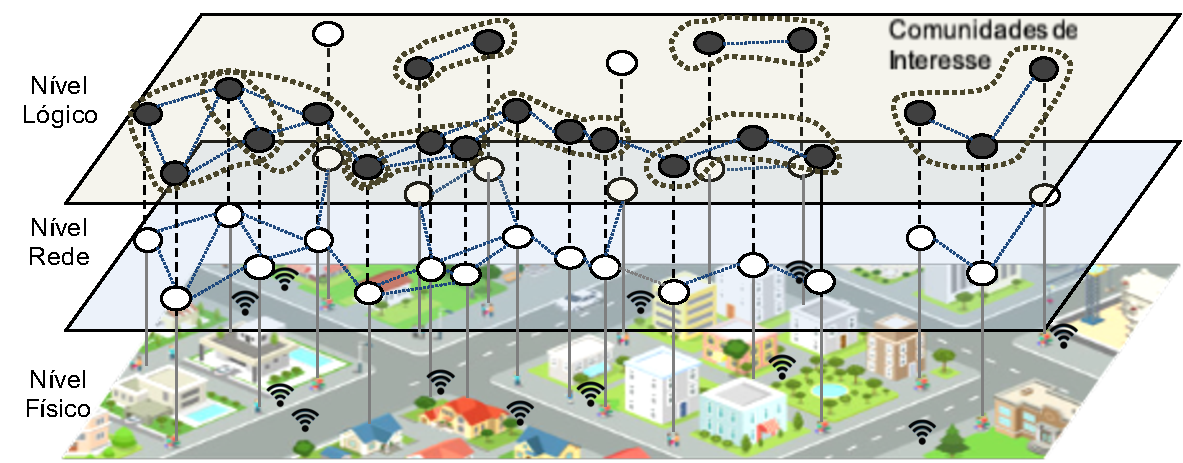
\includegraphics[width=1\textwidth]{figures/ModeloRede.pdf}
\caption{Modelo de Rede}
\label{fig:modeloRede}
\end{figure}
\end{minipage}
\begin{minipage}[b]{.52\linewidth}
\begin{figure}[H]
\centering
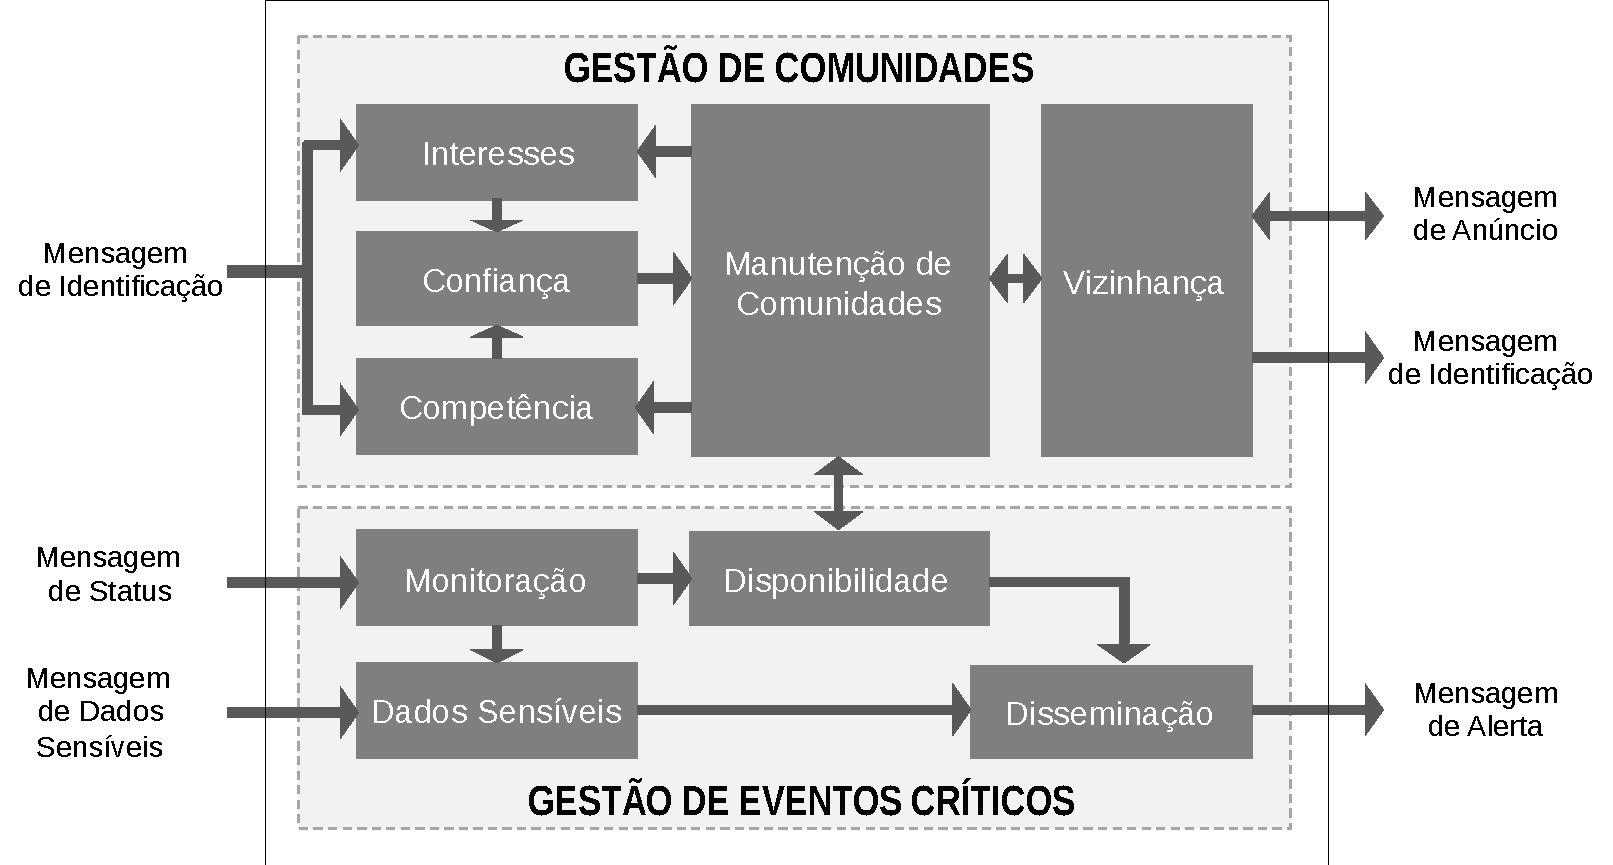
\includegraphics[width=1\textwidth]{figures/Arquitetura_8_p.pdf}
\caption{Arquitetura do STEALTH}
\label{fig:ArquiteturaStealth}
\end{figure}
\end{minipage}
%\end{comment}

O funcionamento do \mbox{STEALTH} inicia com os nós da rede operando de forma isolada e, na medida em que se movimentam, encontram outros nós e estabelecem comunidades de interesse. Periodicamente, cada nó inicializa sua lista de vizinhos, anuncia sua presença por mensagens de anúncios em \textit{broadcast} à procura de nós vizinhos e aguarda um intervalo de tempo até um novo anúncio.  Quando um nó vizinho percebe que um nó anuncia a sua presença, encaminha a este nó anunciador uma mensagem de identificação, composta pela seu \textit{Id}, competência e interesses. O nó anunciador, ao receber essa mensagem do nó vizinho, verifica a existência de interesse em comum em saúde entre eles. Quando há esse interesse,
%em comum, 
ele mede a confiança do nó vizinho e o insere na sua lista de vizinhos, dentro da sua comunidade de saúde. A partir
%da confiança do nó vizinho acerca dos interesses em comum que eles possuem
dessa confiança~(Eq.~\ref{eq:communityTrust}) e da sua competência~(Eq.~\ref{eq:SkillTrust}), obtém-se a confiança total do nó~(Eq.~\ref{eq:totalTrust}). 
%Essas equações estão detalhadas na dissertação.
%
Nas situações emergenciais de saúde, os nós pertencentes às CoI 
%formadas 
%com interesse 
em saúde apoiam os nós que representam pessoas em situação emergencial. Assim, ao ocorrer um evento crítico com um 
%determinado 
nó, este nó determina o nó vizinho 
que ele mais confia, e o dado sensível apropriado a ser disseminado. Em seguida, ele envia uma mensagem de alerta ao nó selecionado com seu dado sensível, e anuncia aos nós
%por \textit{broadcast} 
a interrupção de sua operação. Ao receber uma mensagem de alerta, o nó confirma seu recebimento. Quando um nó percebe que outro nó anuncia a interrupção de sua operação, ele exclui esse nó da sua lista de vizinhos. Isso impede que um nó em situação emergencial seja selecionado para receber dados sensíveis de outros nós. 


\vspace{-0.5cm}

\noindent
\begin{minipage}{.3\linewidth}
\centering
\begin{equation}
T_{xy}^{I} = \frac {|I_x \cap I_y|}{|I_x|}
\label{eq:communityTrust}
\end{equation}
%\hspace{0.5cm}
\end{minipage}
\begin{minipage}{.3\linewidth}
\centering
\begin{equation}
T_{xy}^{Skill} = Sim_y
\label{eq:SkillTrust}
\end{equation}
\end{minipage}
\hspace{0.5cm}
\begin{minipage}{.3\linewidth}
\centering
\begin{equation}
T_{xy} = \frac{T_{xy}^{I} + T_{xy}^{Skill}}{2}
\label{eq:totalTrust}
\end{equation}
\end{minipage}


%\subsection{Funcionamento}
%Esta seção ilustra o funcionamento do sistema e demonstra sua contribuição na disseminação sob controle dos dados sensíveis de uma pessoa em situação emergencial, a fim de que ela possa receber um primeiro atendimento. 
Nós ilustramos a operação do \mbox{STEALTH} em um ambiente urbano de modo a apoiar uma pessoa em situação emergencial, a fim de que ela possa receber um primeiro atendimento.
 \rev{Considere uma área urbana onde seis pessoas deslocam-se a pé pelas ruas: uma enfermeira, um paciente, um executivo, um policial, um bombeiro e um médico. Cada uma delas possui uma profissão ou habilidade para executar determinadas tarefas no seu dia-a-dia. O paciente é uma pessoa que eventualmente precisa de atendimento emergencial. O médico 
 %são profissionais que 
 detém o maior conhecimento em saúde e o policial, por exemplo, possui condições de prestar primeiros socorros.}
%
\rev{Todas essas pessoas} possuem um interesse em comum em saúde e não mantêm relações entre si, mas podem estabelecer
{\bf redes locais dinâmicas} em razão
%das suas proximidades 
da sua proximidade
e do interesse em saúde. 
%A enfermeira, o policial, o bombeiro e o médico possuem interesse em saúde por conta da sua profissão. O executivo se interessa por saúde, por exemplo, a fim de ajudar pessoas necessitadas. 
As pessoas portam dispositivos móveis, \textit{smartphones}, para se conectarem em redes. O \mbox{STEALTH} roda nesses \textit{smartphones}. 
%, estando configurado para operar. 
Além disso, o paciente porta um dispositivo junto ao seu corpo para verificar sua pressão arterial, por exemplo, e reportar a um aplicativo instalado em seu \textit{smartphone}. Esse aplicativo comunica-se com o \mbox{STEALTH} 
%informando 
para informar 
os valores de pressão arterial medidos e sua normalidade para esse paciente.


\begin{table}[!htb]
	\begin{minipage}[t]{0.5\linewidth}
		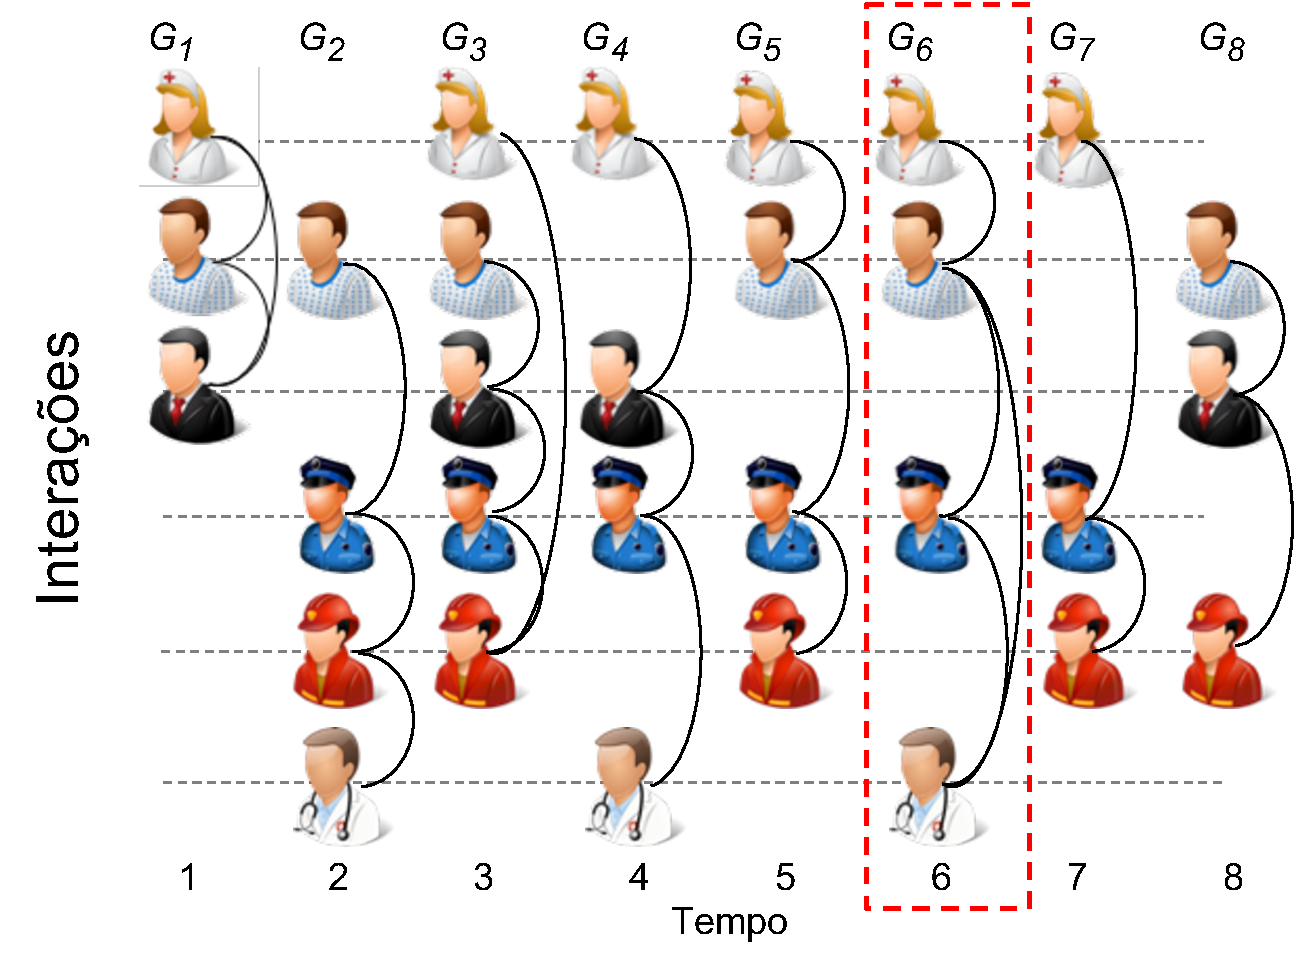
\includegraphics[width=0.95\textwidth]{figures/interacoes_t6.pdf}
		\captionof{figure}{Interações no tempo}
		\label{fig:interacoesnotempo}
	\end{minipage}
	\begin{minipage}[b]{0.5\linewidth}
		\centering
		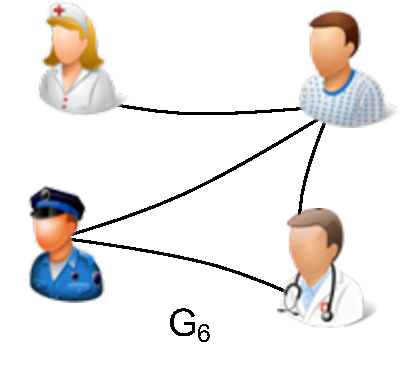
\includegraphics[width=.3\textwidth]{figures/Grafo6.pdf}
		\vspace{-0.2cm}
		\captionof{figure}{Grafo da rede em $t_6$}
	    \label{fig:grafo6}
	    \relsize{-2.0}
	    \captionof{table}{Medição da confiança}
        \label{tab:exemploConfianca2}
        {
            \begin{tabular}{|l|ccc|}
            \hlineB{2}
            \multirow{2}{*}{\textbf{Confiança}}&\multicolumn{3}{c|}{\textbf{Competência}}  \\ \cline{2-4}  %\bigstrut \\ \cline{2-4} 
            &Médico&Enfermeira&Policial  \\ \hline %\bigstrut \\ \hline
            \textbf{$T^{Skill}$}&1&0,33&0,28 \\ % \bigstrut \\
            \textbf{$T^{CoI}$}&1&1&1  \\ %\bigstrut \\
            \textbf{$T$}&1&0,66&0,64 \\ % \bigstrut \\
            \hlineB{2}
            \end{tabular}
        }
	\end{minipage}\hfill
\end{table}

%\vspace{-0.5cm}

As interações entre pessoas ao longo do tempo $t = \{1,2,...,8\}$, resultantes da sua mobilidade, estabelecem redes locais, ilustradas na Figura \ref{fig:interacoesnotempo}, quando seus dispositivos estabelecem redes \textit{ad hoc} para trocarem dados entre si. Assume-se que o paciente entra em uma situação emergencial em $t_6$. Nesse instante, o seu dispositivo interage com os de outras pessoas próximas, como ilustra o grafo temporal $G_6$ (Figura \ref{fig:grafo6}), e cada um deles forma sua própria comunidade de saúde. O dispositivo do paciente mede a confiança dos demais e os insere entre os seus 
%na sua lista de 
vizinhos com os valores de confiança exibidos na  Tabela~\ref{tab:exemploConfianca2}. Ao ocorrer o evento crítico em $t_6$, \rev{o STEALTH rodando no \textit{smartphone} do} paciente recomenda o médico como 
%a pessoa com 
o maior valor de confiança na sua comunidade de saúde e, assim, dissemina seus dados sensíveis
%de modo 
para
que ele possa
%tomar 
adotar
alguma ação.

%\vspace{-0.5cm}
\section{Avaliação} % do STEALTH}
\label{sec:aval}

O sistema \mbox{STEALTH} foi implementado e simulado no simulador NS-3, versão 3.28.\footnote{Código disponível em https://github.com/agnaldosb/stealth}
%\as{[RODAPE para o codigo]} 
Todos os resultados correspondem à média de 35 simulações, com intervalo de confiança de 95\%. 
%A Tabela~\ref{tab:parametros} sintetiza os principais parâmetros empregados nas simulações. 
A análise da disponibilidade dos dados provida pelo \mbox{STEALTH} levou em conta a evolução das comunidades de interesse em saúde ao longo do tempo e a métrica \textit{Número médio de comunidades de interesse em saúde}~($N_{C}$). A análise da confiabilidade é mensurada através das métricas \textit{Taxa de sucesso no acesso aos dados}~($TS$), \textit{Taxa de dados não acessados}~($TN_a$), \textit{Tempo médico de acesso aos dados}~($MTA$) e \textit{Taxa de sucesso no acesso aos dados por competência}~($TS_{Skill}$).
Os parâmetros empregados nas simulações, bem como todos os resultados obtidos estão na dissertação.
%A Tabela~\ref{tab:metricas} descreve as métricas utilizadas se encontram detalhadas na dissertação.

Os nós da rede foram configurados randomicamente com aspectos sociais a cada repetição de simulação, conforme Tabela~\ref{tab:aspectosAtribuidos}, possuindo uma única competência e um conjunto de interesses, com um mínimo de um e máximo cinco interesses.
%A Tabela~\ref{tab:aspectosAtribuidos} lista a distribuição dos aspectos. 
A avaliação
%do comportamento 
do sistema foi realizada
%através 
por meio
%de três nós - 
dos nós
37, 52 e 70. Cada um desses nós recebeu a mesma configuração em todas as repetições de simulações e entrou em situação emergencial aos 890s. Assumiu-se que todos os nós %apresentam 
possuem 
um comportamento honesto e há mecanismos de segurança para validar suas identidades e proteção na transmissão dos dados. \rev{Assume-se, 
%também, 
que o alerta de um evento crítico acontece por meio de um dispositivo portado pelas pessoas junto ao seu corpo, e que informa ao \mbox{STEALTH}.}



\begin{comment}

\begin{table}[H]
\setlength{\extrarowheight}{2.0pt}
\relsize{-1.0}
\centering
\caption{Principais parâmetros de simulação}
\label{tab:parametros}
\begin{tabular}{|ll||ll|}
\hlineB{2}
\textbf{Parâmetro} & \textbf{Valor} & \textbf{Parâmetro} & \textbf{Valor} \\ \hline
Quantidade de nós & 100 & Raio de transmissão & 50m \\
Tempo de simulação & 900s & Padrão de comunicação & IEEE 802.11a\\
Área de movimentação & 400m x 430m & Protocolo & UDP\\
Velocidade dos nós & 0,5m/s e 2,0m/s && \\
\hlineB{2}
\end{tabular}
\end{table}

\end{comment}


%, instalado no sistema operacional Debian, versão 9.1. O cenário de uso do \mbox{STEALTH} é composto por 100 dispositivos (nós) móveis representando o comportamento de movimentação de usuários em um ambiente urbano. Esses usuários portam equipamentos sem fio - \textit{smartphones} - e deslocam-se em uma área de 400m x 430m da Cidade de Estocolmo (Suécia) com velocidades entre 0,5m/s e 2,0m/s~\cite{helgason2014opportunistic}. Os nós estabelecem redes \textit{ad hoc} através de transmissão usando o padrão IEEE 802.11a e o protocolo de transporte UDP. O raio de alcance dos nós é de 50m, para permitir a \rev{formação de comunidades} de interesses ao seu redor e na medida em que se movimentam. Além disso, eles são configurados randomicamente com aspectos sociais, isto é, a cada repetição de simulação eles possuem uma única competência e um conjunto de interesses, com um mínimo de um e máximo cinco interesses. A Tabela~\ref{tab:aspectosAtribuidos} lista a distribuição dos aspectos. A classe \textit{node} do NS-3 foi modificada para incorporar os atributos sociais de confiança aos nós.


\begin{comment}


\as{mencionar as métricas no texto e seus acrônimos e remover a tabela de métricas}

\begin{table}[H]
\renewcommand*{\arraystretch}{2.0}
\centering
\caption{Métricas de avaliação de desempenho}
\label{tab:metricas}
{\footnotesize
\begin{tabular}{|l|c|l|}
\hlineB{2}
\textbf{Métrica} &\textbf{Representação} & \textbf{Descrição} \\ \hline

$N_{C}$ & $\mathlarger{\sum}\limits_{i\;=\;1}^{N_S} \; \mathlarger{\sum}\limits_{j\;=\;1}^{t_s} \; \dfrac{ C_{xy}}{t_s \; \times \; N_S}$  & Número médio de comunidades de interesse em saúde estabelecidas \\

$TS$ & $\dfrac{A_{Success}}{A_{Disp}} \times 100$ & Taxa de sucesso no acesso aos dados sensíveis\\

$TS_{Skill}$ & $\dfrac{A_{Skill}}{A_{Success}} \times 100$ & Taxa de sucesso no acesso aos dados sensíveis por competência\\

$TN_a$ & $100 - TS$ & Taxa de dados sensíveis não acessados\\ 

$MTA$ & $\mathlarger{\sum}\limits_{i\;=\;1}^{N_S} \; \dfrac{ ta_i - td_i}{N_S}$  & Tempo médio de acesso aos dados sensíveis\\ \hlineB{2}
\end{tabular}
}
\end{table}
\end{comment}

\begin{table}[H]
\setlength{\extrarowheight}{2.0pt}
\relsize{-2.0}
\centering
\caption{Distribuição dos aspectos sociais atribuídos aos nós}
\vspace{-0.2cm}
\label{tab:aspectosAtribuidos}
\begin{tabular}{|l|cccc|ccccc|}
\hlineB{2}
\multirow{2}{*}{\textbf{Aspectos Sociais}} & \multicolumn{4}{c|}{\textbf{Competências}} & \multicolumn{5}{c|}{\textbf{Interesses}} \\ \cline{2-10}
&Médico&Enfermeiro&Cuidador&Outras&Saúde&Turismo&Música&Filmes&Livros \\ \hline
\textbf{\# de Nós} &10&15&20&55&20&30&45&60&15 \\ 
\hlineB{2}
\end{tabular}
\end{table}

\begin{comment}

\begin{table}[!htb]
\renewcommand*{\arraystretch}{1.4}
\centering
\caption{Métricas de avaliação de desempenho}
\vspace{-0.2cm}
\label{tab:metricas}
{ \footnotesize
\begin{tabular}{m{10cm}cm{4cm}}
\hlineB{2}
\textbf{Descrição} & \textbf{Equação} \\ \hline

\textbf{\textit{Número Médio de Comunidades de Interesse em Saúde}} ($N_{C}$) computa a média do somatório de todas as comunidades de saúde formadas por um nó ao longo de todas 
\rev{as execuções ($N_S$).} & $N_{C} = \mathlarger{\sum}\limits_{i\;=\;1}^{N_S} \; \mathlarger{\sum}\limits_{j\;=\;1}^{t_s} \; \dfrac{ C_{xy}}{t_s \; \times \; N_S}$ \\

\textbf{\textit{Taxa de Sucesso no Acesso aos Dados}} ($TS$) indica a taxa de sucesso na entrega dos dados à pessoa adequada, sendo a razão entre o total de acessos com sucesso aos dados sensíveis ($A_{Sucess}$) e o total de vezes em que os dados sensíveis estiveram disponíveis para acesso ($A_{Disp}$). & $TS = \dfrac{A_{Success}}{A_{Disp}} \times 100$ \\

\textbf{\textit{Taxa de Sucesso no Acesso aos Dados por Competência}} ($TS_{Skill}$) equivale à métrica $TS$ computada pela razão entre o acesso de \rev{cada competência individualmente ($A_{Skill}$) e o total de acessos com sucesso ($A_{Success}$)}, diante das competências vistas na Tabela~\ref{tab:aspectosAtribuidos}. & $TS_{Skill} = \dfrac{A_{Skill}}{A_{Success}} \times 100$ \\

\textbf{\textit{Taxa de Dados Não Acessados}} ($TN_a$) corresponde ao porcentual de dados que não foram acessados nas situações emergenciais. & $TN_a = 100 - TS$ \\ 

\textbf{\textit{Tempo Médio de Acesso aos Dados Sensíveis}} ($MTA$) computa o tempo médio de acesso aos dados sensíveis de um determinado nó para todas as simulações realizadas. Ele corresponde ao somatório da razão entre as diferenças entre o momento em que os dados foram acessados ($t_r$) e o momento da sua disseminação ($t_s$) e o \rev{total de execuções} ($N_S$). & $MTA = \mathlarger{\sum}\limits_{i\;=\;1}^{N_S} \; \dfrac{ ta_i - td_i}{N_S}$ \\ \hlineB{2}
\end{tabular}
}
\end{table}
\end{comment}


\begin{comment}



A avaliação do comportamento do sistema foi realizada através de três nós - 37, 52 e 70.
%Para isso, eles 
%Eles
%receberam 
Cada um desses nós recebeu
a mesma configuração
%cada um 
em todas as repetições de simulações e
%, enquanto os demais nós foram configurados randomicamente a cada repetição de simulação. 
entrou em situação emergencial aos 890s.
%de simulação.
%, permitindo observar seus comportamentos em grande parte da simulação. 
Assumiu-se que todos os nós apresentam um comportamento honesto
e há mecanismos de segurança para validação das suas identidades e proteção na transmissão dos dados. \rev{Assume-se, também, que a identificação de um evento crítico 
acontece 
por meio de um dispositivo que as pessoas 
portam 
junto ao seu corpo, e que informa ao \mbox{STEALTH}.}
%Os resultados exibidos correspondem à média de 35 simulações e um intervalo de confiança de~95\%.

%As métricas  empregadas  na avaliação de desempenho do sistema \mbox{STEALTH} são detalhadas na Tabela~\ref{tab:metricas} e foram definidas especificamente para essa finalidade. 

\end{comment}


%\section{Resultados obtidos}
%\section{Resultados de 
\section{Disponibilidade e Confiabilidade}
\label{sec:results}

%Esta seção apresenta os resultados obtidos ao longo das simulações, quando foi verificada a disponibilidade e confiabilidade do \mbox{STEALTH} na disseminação controlada de dados sensíveis. Na dissertação discute-se esses e outros resultados em detalhes.

%\subsection{Disponibilidade}

\begin{wrapfigure}{r}{0.35\textwidth}
\centering
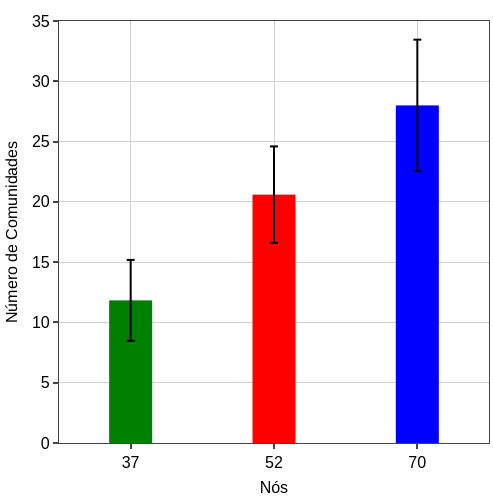
\includegraphics[width=.35\textwidth]{figures/coi_mean_performance_3_SBSEG19_v2.png}
\vspace{-0.5cm}
\caption[Número médio de comunidades]
{\tabular[t]{@{}l@{}}Número médio de \\ comunidades\endtabular}
\label{fig:coiEstabelecidas}
\end{wrapfigure}    

A
%análise da 
disponibilidade
do STEALTH
%verifica a 
representa sua
prontidão
%do sistema 
para disseminar com sucesso e de modo controlado os dados sensíveis das pessoas em situação emergencial.
%A Figura~\ref{fig:coiEstabelecidas} demonstra esse 
%Esse
%comportamento ao sintetizar o 
O
número médio de comunidades de interesse em saúde ($N_{C}$) demonstra esse comportamento (Figura~\ref{fig:coiEstabelecidas}).
%estabelecidas ao longo do tempo. 
O nó 37 estabeleceu, em média, 12 CoI
%distintas ao longo de 
em
cada repetição de simulação,
%. Isso caracteriza 
caracterizando
a dinamicidade das redes locais estabelecidas
%, especialmente da
e de sua topologia. A mobilidade dos nós,
%através de caminhos dis\-tintos, 
associada aos seus aspectos sociais (interesses),
%- atribuídos a eles, 
impactou a formação
%dessas 
das
comunidades. O nó 70 estabeleceu uma quantidade
%ainda 
maior de comunidades, $N_C$ = 28,
%o que aumenta 
elevando
a disponibilidade para disseminação de seus dados em situações emergenciais.

A
evolução
%dinamicidade e o tamanho
%A Figura~\ref{fig:neighs_x_cois} apresenta os gráficos da dinamicidade 
das comunidades de saúde dos nós 37, 52 e 70, estabelecidas pelo \mbox{STEALTH}
%e seu tamanho 
%ao longo do tempo 
em uma repetição específica de simulação, é ilustrada na Figura~\ref{fig:neighs_x_cois}.
%Os resultados mostram 
%Observa-se que o \mbox{STEALTH} 
O \mbox{STEALTH} acompanhou 
a dinamicidade das redes locais criadas diante da mobilidade dos nós, ajustando suas CoI.
%. Ele verificou as mudanças nas vizinhanças dos nós e ajustou suas CoI. 
O nó 37 formou comunidades em 63,93\% do tempo em que esteve ativo. Nesse período, o sistema esteve apto para disseminar seus dados sensíveis, pois  identificou  vizinhos que poderiam auxiliá-lo. Contudo,
ao entrar em emergência aos 890s, o nó 37 não possuía vizinhos ao redor, impedindo a formação de uma comunidade e  a disseminação de seus dados sensíveis. O nó 52 manteve um comportamento distinto  e estabeleceu comunidades em 97,22\% do tempo, até que entrou em situação emergencial. Neste instante, como se observa na Figura~\ref{fig:neighs_x_cois}, ele possuía sete vizinhos, mas apenas dois deles pertenciam a sua comunidade de saúde (i.e., nós 13 e 41). 
Em razão do nó 13 possuir  uma competência mais elevada em saúde, \textit{cuidador}, o nó 52 disseminou seus dados para ele. Já  o nó 70  formou comunidades de saúde por mais tempo, 98,8\%. Esse comportamento é confirmado pela Figura~\ref{fig:coiEstabelecidas}, onde o nó 37 estabeleceu o menor $N_C$, 12, e o nó 70 teve o maior valor entre todos os nós, 28. Ao entrar em emergência, o nó 70 tinha 4 vizinhos, mas apenas um deles com interesse em saúde - nó 96, para o qual seus dados sensíveis foram disseminados. 

\begin{figure}[!htb]
\centering
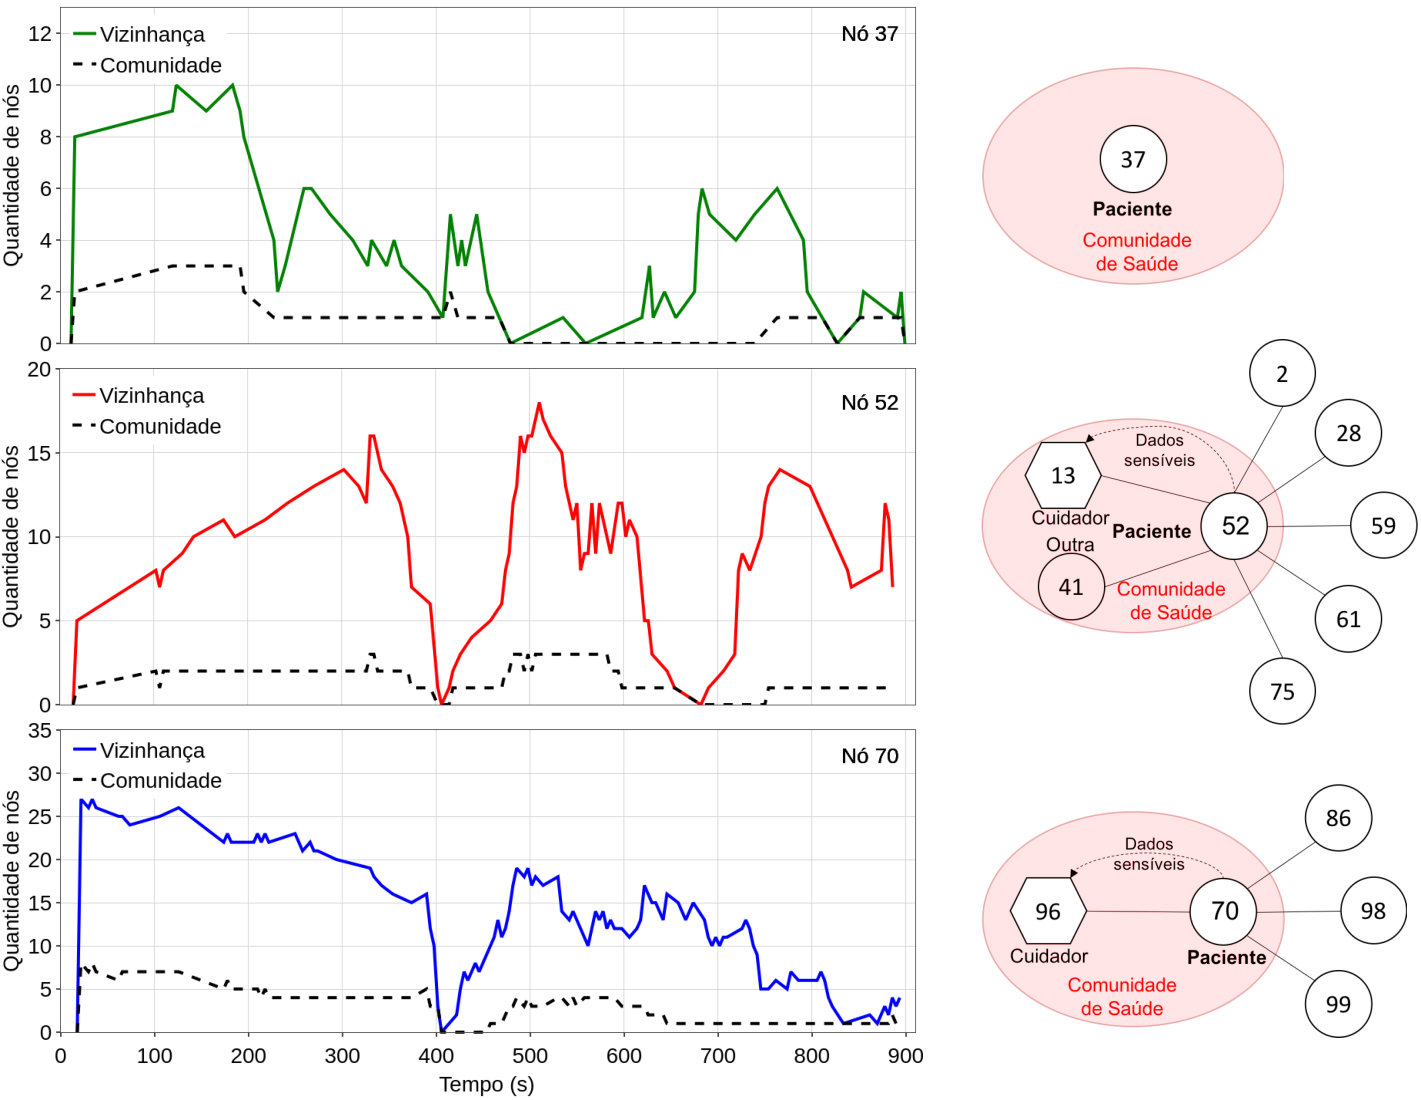
\includegraphics[width=0.9\textwidth]{figures/neighs_cois_v2_890s_stack_3.pdf}
\vspace{-0.2cm}
\caption{Dinamicidade e tamanho da comunidade de saúde ao longo do tempo}
\label{fig:neighs_x_cois}
\end{figure}

%\subsection{Confiabilidade}

A análise da confiabilidade 
leva em conta
%verifica 
a capacidade do sistema em disseminar com sucesso e de modo controlado os dados sensíveis das pessoas em situação emergencial.
%O comportamento dos nós selecionados - 37, 52 e 70 - demonstra essa situação. 
O nó 52 foi bem-sucedido ($TS$) na disseminação de seus dados sensíveis em 80\% das situações emergenciais ao longo das repetições de simulações.
%, quando seus dados disseminados foram acessados com sucesso. 
O agrupamento dos nós em comunidades de interesse impacta
%diretamente 
a $TS$, pois garante a disseminação dos dados sensíveis de um nó em situação emergencial apenas a um outro nó dentre aqueles
%que pertençam à
pertencentes a sua CoI em saúde. A importância das comunidades no controle da
disseminação
desses dados
%dos dados sensíveis
%dos nós 
é constatada pelos dados não acessados ($TNa$). 
%Em 68,57\% das situações emergenciais, os dados sensíveis do nó 37 não foram acessados por outros nós. 
Os dados sensíveis do nó 37 não foram acessados em 68,57\% das situações emergenciais.
%Isso ocorreu devido à 
Isso se deve à
falta de uma comunidade de saúde durante as situações emergenciais ou 
%por conta da sua 
a sua mobilidade, que interrompeu a conexão com os outros nós da sua rede local.
%foi interrompida por conta da sua mobilidade. 
\rev{O nó 70 não foi tão bem-sucedido quanto o nó 52, apesar de ter estabelecido um maior número de comunidades, como 
%se observa 
visto na Figura~\ref{fig:coiEstabelecidas}.
%Isso se deve ao 
%ocorreu por conta de que no 
Isto deve-se 
%A causa desse desempenho foi a
a falta  de vizinhos
%Geralmente, 
no instante em que o nó 70 entrou em situação emergencial nas repetições de simulações.
%quando 
%Como não haviam 
A ausência de 
vizinhos para formar uma comunidade de saúde  %possuir 
%existia vizinhos na sua comunidade de saúde para os quais pudesse disseminar seus dados.
tornou a disseminação de seus dados sensíveis inviável.} 
%
O tempo médio de acesso aos dados sensíveis (\textbf{$MTA$}) representa o custo em relação ao tempo para que os dados sensíveis disseminados por um nó em situação emergencial sejam acessados.
%Ele
%é impactado diretamente pela 
%sofre impacto da
A
dinamicidade das redes locais estabelecidas
impacta o \textbf{$MTA$}, visto que
%, cuja 
a mobilidade dos nós impõe mudanças à
topologia dessas redes.
%se modifica com a mobilidade dos nós. 
%A 
Os resultados 
%apresentados 
na
Tabela~\ref{tab:AcessoCompetencia} demonstram que o STEALTH dissemina dados sensíveis
%sumariza os resultados obtidos, onde se
%é possível 
%constata 
%que eles 
atendendo à latência máxima de 125ms estabelecida pela IEEE para entrega de alertas médicos~\cite{ieee2012}.
%Os 
O acesso aos
dados sensíveis do nó 52
%foram acessados
%imediatamente 
\rev{deu-se mais rapidamente que para os dos demais nós
($MTA$~<~1ms)}, já os do nó 37 foram acessados, em média, após 95ms de sua disseminação. As CoI contribuem
%para o processo de \rev{tomada de decisão}
nas tomadas de decisões
%sobre o 
acerca do
nó adequado 
que terá acesso aos dados disseminados, além de
%e reduzem 
reduzirem
o tempo de acesso a esses dados.

\begin{table}[!htb]
	\begin{minipage}[t]{0.5\linewidth}
	    \centering
        \caption{Disseminação dos dados}
        \vspace{-0.2cm}
        \label{tab:AcessoCompetencia}
        { \footnotesize
        \begin{tabular}{l|c|ccc}
        \hlineB{2}
        \multicolumn{2}{l|}{\textbf{Métrica}} & $TS$ &$TN_a$& $MTA$\bigstrut \\ \hline %\hline
        \multirow{3}{*}{\textbf{Nó}}&37 & 31,43\% &\textcolor{blue}{\textbf{68,57}\%}& \textcolor{blue}{\textbf{95 ms}}\bigstrut \\ 
        &52 & \textcolor{blue}{\textbf{80,00}\%} &20,00\% & \rev{< 1ms}\bigstrut \\
        &70 & 60,00\% &40,00\% &2,3 ms \bigstrut \\ 
        \hlineB{2}
        \end{tabular}
        }
	\end{minipage}	
	\begin{minipage}[t]{0.5\linewidth}
	    \centering
	    \relsize{-2.0}
        \caption{Controle de disseminação}
        \vspace{-0.2cm}
        \label{tab:taxaMedia}
        { \footnotesize
        \begin{tabular}{l|c|c}
        \hlineB{2}
        \multicolumn{2}{l|}{\textbf{Métrica}} & $TS_{Skill}$ \bigstrut \\ \hline
        \multirow{4}{*}{\textbf{Competência}}&Médico & 30,03\% \bigstrut \\
        &Enfermeiro & 39,40\% \bigstrut \\
        &Cuidador & 9,09\% \bigstrut \\ 
        \hlineB{2}
        \end{tabular}
        }
	\end{minipage}\hfill
\end{table}

\vspace{0.3cm}

Os dados sensíveis dos nós em situação emergencial foram disseminados pelo \mbox{STEALTH} apenas aos nós pertencentes as suas comunidades de saúde e diante das competências vistas na Tabela~\ref{tab:aspectosAtribuidos}.
%O emprego de 
Os
interesses e competências, associados
%à formação de 
às
comunidades de interesse, além de possibilitarem avaliar a confiança dos nós, também permitem controlar a disseminação dos seus dados sensíveis. Isso ocorre em uma condição \textit{Zero-Knowledge}, visto que as comunidades de saúde são recriadas periodicamente, desconsiderando interações anteriores entre os nós da rede. O sucesso no acesso aos dados por competência ($TS_{Skill}$)
%indica a
comprova a
%prevalência 
importância
das competências nas comunidades estabelecidas. 
Através da Tabela~\ref{tab:taxaMedia}, observa-se
%que
%\al{21,48\% do total de dados disseminados foram para nós com outras competências, enquanto  
%30,03\% dos dados sensíveis foram acessados por nós com competência de \textit{médico},
%. Isso indica 
%indicando
%um \textit{médico} acessou 
que os \textit{médicos} acessaram os
dados sensíveis
em 30,03\% das situações emergenciais.
%Logo, nesses 
Nesses
momentos,
o \mbox{STEALTH} detectou a presença de pelo menos um \textit{médico} na comunidade de saúde dos nós avaliados.

\vspace{-0.2cm}

\section{Conclusão}
\label{sec:conc}

Esta dissertação apresentou \mbox{STEALTH}, um sistema para disseminar dados sensíveis de saúde de forma controlada em redes locais dinâmicas sem fio. Ele estabelece agrupamentos virtuais levando em conta comunidades de interesses e aplica confiança social a fim de permitir aos dispositivos decidirem de maneira robusta num dado momento sobre a disseminação de dados diante de uma situação emergencial. Uma avaliação do STEALTH num ambiente realístico mostrou a sua eficácia ao antecipar a identificação de pessoas próximas para auxiliar em eventos críticos de saúde, e sua confiabilidade na disseminação controlada dos dados sensíveis das pessoas em situação emergencial. As contribuições deste trabalho resultaram na publicação~\cite{batista2019sbseg}.

\small
\bibliographystyle{sbc}
\bibliography{sbc-template}

\end{document}

